\chapter{Technical approach}

The proposed two-stream approach consists of an appearance
stream, representing the static (texture) appearance of each frame,
and a dynamics stream, representing temporal 
variations between frames.
Each stream consists of a ConvNet whose activation 
statistics are used to characterize the dynamic texture.
Synthesizing a dynamic texture is formulated as an optimization 
problem with the objective of matching activation 
statistics between the target and synthesized textures.
The dynamic texture synthesis approach is summarized in Fig.\ \ref{fig:architecture}
and the individual pieces are described in turn in the
following sections.

\begin{figure}[t]
\begin{center}
    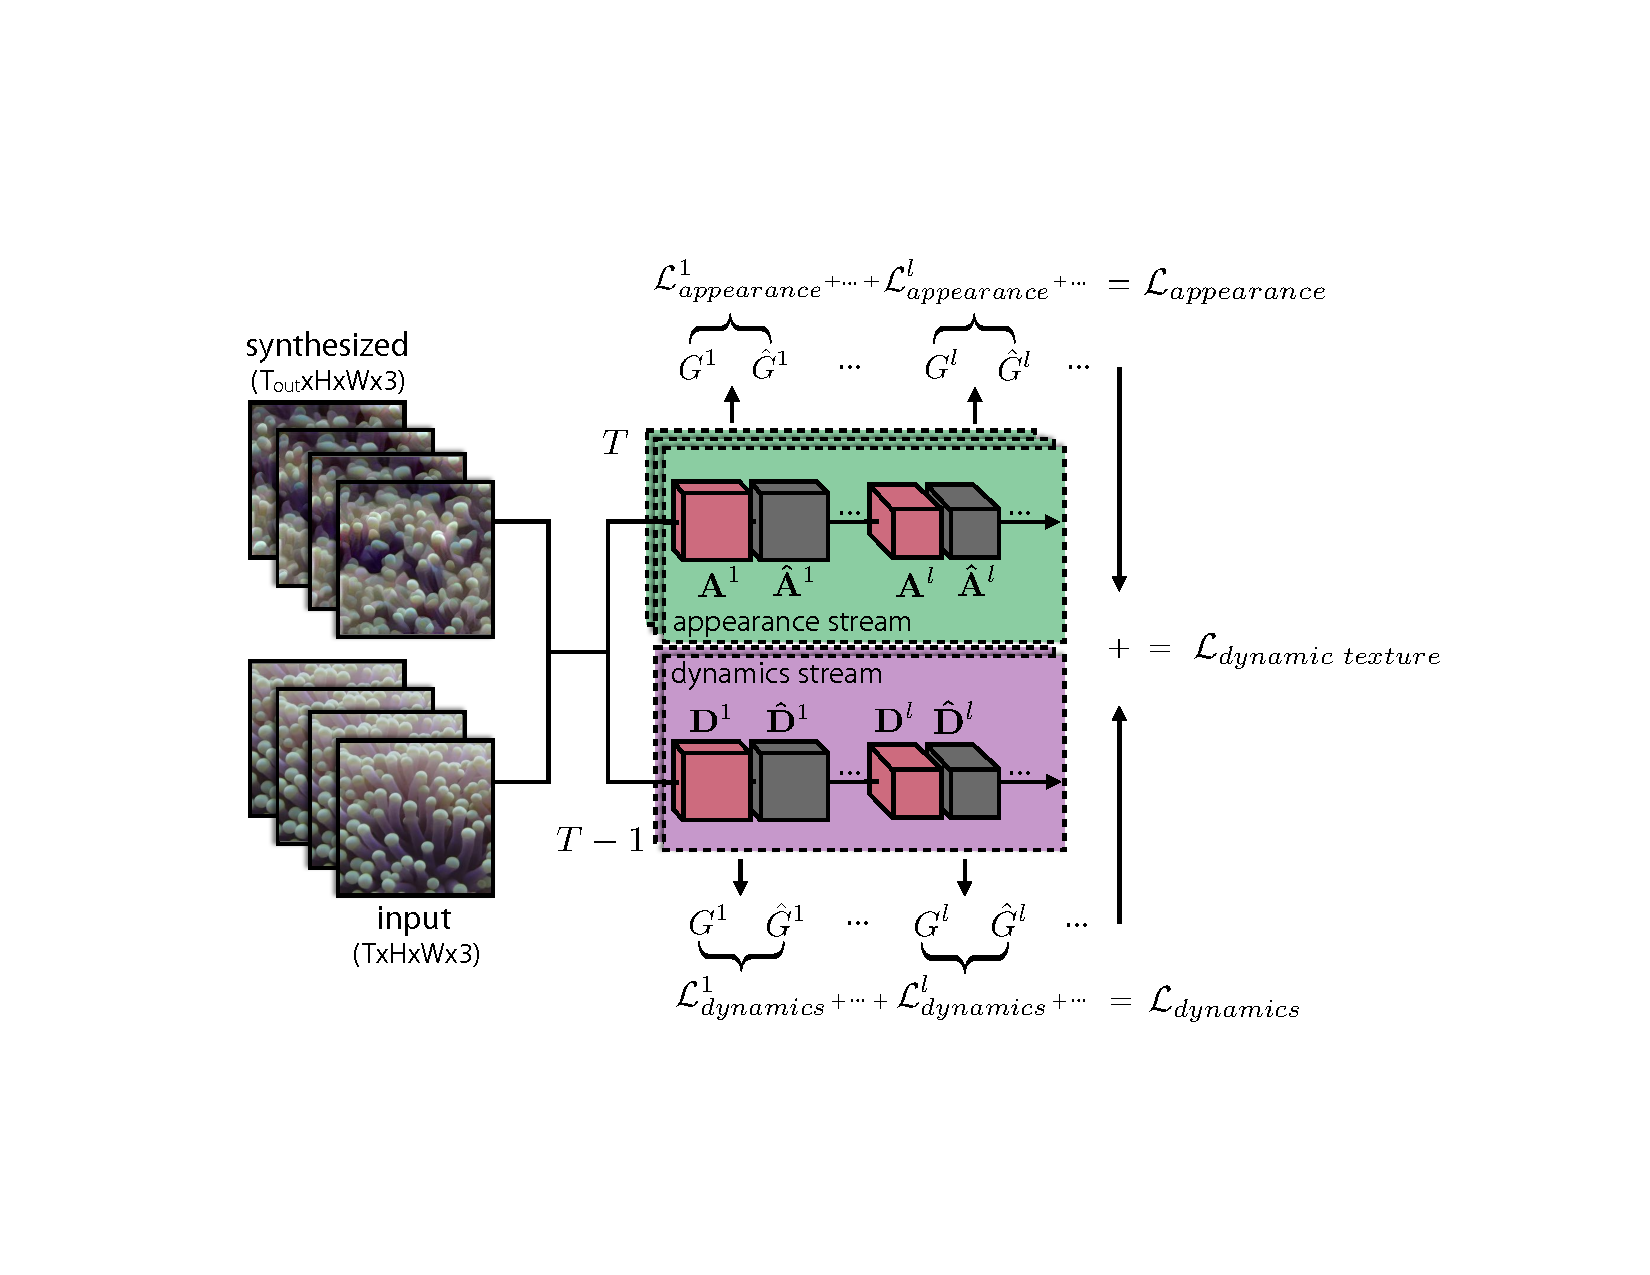
\epsfig{file=overallarchitecture.pdf, width = \textwidth}
\end{center}
\vspace{-0.45cm}
\caption[Two-stream dynamic texture generation.]{Two-stream dynamic texture generation.
Two sets of Gram matrices represent a dynamic texture's appearance and 
dynamics.
Matching these statistics allows for the generation of novel
textures as well as style transfer between textures. Here, $G^l$ and $\hat{G}^l$ are the Gram matrices of activations $A^l$ and $\hat{A}^l$ (or $D^l$ and $\hat{D}^l$) corresponding to the target and synthesized sequence, respectively, computed at layer $l$ of the appearance stream (or dynamics stream) and averaged over time $T$ (or $T-1$). $\mathcal{L}_\text{appearance}^l$ is the appearance loss at layer $l$, computed as the squared Frobenius norm between $G^l$ and $\hat{G}^l$ from the appearance stream. Similarly, $\mathcal{L}_\text{dynamics}^l$ is the dynamics loss at layer $l$ for the dynamics stream. By summing each loss computed at various layers, we arrive at $\mathcal{L}_\text{appearance}$ and $\mathcal{L}_\text{dynamics}$, which, when summed, form the combined dynamic texture loss, $\mathcal{L}_\text{dynamic texture}$, that is to be minimized.}
\label{fig:architecture}
\end{figure}


\section{Texture model: Appearance stream}

The appearance stream follows the static texture model
introduced by Gatys \etal \cite{gatys2015} which was summarized in the previous chapter (Sec.\ \ref{sec:texture_synthesis_using_a_convnet}).
To briefly review, the key idea is that correlations between activation maps (\ie, normalized Gram matrices) in a 
ConvNet trained for 
object recognition (\eg, VGG-19 \cite{simonyan2014very}) 
capture texture appearance.
The same publicly available normalized VGG-19 ConvNet \cite{simonyan2014very} used by Gatys \etal \cite{gatys2015} is used here. The proposed appearance stream utilizes this model by simply applying it indepedently to each frame of the synthesized and target texture.

\subsection{Target texture appearance}

To capture the appearance of an input dynamic texture, an initial forward pass through VGG-19 is performed with each frame of the image sequence to compute the feature activations (filter responses),
$\mathbf{A}^{lt} \in \mathbb{R}^{N_l\times M_l}$, for various
levels in the network, where $N_l$ and $M_l$ denote
the number of feature activations and the number of spatial locations of layer
$l$ at time $t$, respectively.
The auto-correlations of the filter responses in a particular layer are
averaged over the frames and encapsulated by a Gram matrix,
$\mathbf{G}^{l} \in \mathbb{R}^{N_l \times N_l}$, whose
entries are given by:
\begin{equation}
	G_{ij}^l = \frac{1}{T N_l M_l} \sum_{t=1}^T \sum_{k=1}^{M_l} A_{ik}^{lt} A_{jk}^{lt}\ ,
	\label{eq:gram_target}
\end{equation}
where $T$ denotes the number of input frames
and $A_{ik}^{lt}$ denotes the activation of feature $i$ at
location $k$ in layer $l$ on the target frame $t$.

\subsection{Synthesized texture appearance}

The synthesized texture appearance is similarly represented by a
Gram matrix, $\hat{\mathbf{G}}^{lt} \in \mathbb{R}^{N_l \times N_l}$,
whose activations are given by:
\begin{equation}
	\hat{G}_{ij}^{lt} = \frac{1}{N_l M_l} \sum_{k=1}^{M_l} \hat{A}_{ik}^{lt} \hat{A}_{jk}^{lt}\ ,
	\label{eq:gram_synthesized}	
\end{equation}
where $\hat{A}_{ik}^{lt}$ denotes the activation of feature $i$ at
location $k$ in layer $l$ on the synthesized frame $t$.

\subsection{Appearance loss}

The appearance loss, $\mathcal{L}_\text{appearance}$, is defined as the temporal average of the mean squared error between
the Gram matrix of the input texture and that of the synthesized
texture computed at each frame:
\begin{equation}
   \mathcal{L}_\text{appearance} = \frac{1}{L_\text{app} T_\text{out}} \sum_{t=1}^{T_\text{out}} \sum_{l} \Vert \mathbf{G}^l - \hat{\mathbf{G}}^{lt} \Vert^2_F\ ,
   \label{eq:apploss}
\end{equation}
where $L_\text{app}$ is the number of VGG-19 layers used to compute Gram
matrices, $T_\text{out}$ is the number of frames being generated in
the output, and $\Vert \cdot \Vert_F$ is the Frobenius norm.
Consistent with previous work \cite{gatys2015}, Gram matrices are computed on the
following layers: 
\emph{conv1\_1}, \emph{pool1}, \emph{pool2}, \emph{pool3}, and \emph{pool4}. \highlight{Gatys \etal \cite{gatys2015} found these layers to provide visually-pleasing results for static texture synthesis after they systematically experimented with using other layers. They demonstrated that not all layers of the network are required for visually-pleasing results, so long as the chosen layers span a wide spectrum of receptive fields (\ie, using early, mid, and later layers of the network).}

\section{Texture model: Dynamics stream}

Parallel to the appearance stream ConvNet is a ConvNet designed for capturing texture dynamics. There are three primary goals in designing this dynamics stream.
\begin{enumerate}
	\item The activations of the ConvNet should represent the temporal variation of the input pattern.
	\item The activations should be largely invariant to the appearance (\ie, spatial content) of the images (which should be characterized by the appearance stream described above).
	\item The dynamics representation should be differentiable to enable synthesis via a ConvNet.
\end{enumerate}

By analogy to the appearance stream, an obvious choice
is a ConvNet architecture suited for computing
optical flow (\eg, \cite{dosovitskiy2015,ilg2017}) which
is naturally differentiable.
However, with most such models it is unclear how invariant
their layers are to appearance.
Instead, a novel network architecture is proposed which is
motivated by the spacetime-oriented energy model
\cite{derpanis2012spacetime,simoncelli1998}.

\subsection{Review: Marginalized spacetime oriented energies}

 This section is only intended to briefly review the aspects of the Marginalized Spacetime Oriented Energies (MSOE) model \cite{derpanis2012spacetime} that are most relevant to the following section; a more thorough overview can be found in the previous chapter (Sec.\ \ref{sec:msoe}).

A significant limitation of optical flow is its reliance on a single coherent movement for each pixel and its underlying assumption on brightness constancy, which only partially describes the dynamics one may encounter in the real world, and thus in dynamic textures. In response, Derpanis and Wildes \cite{derpanis2012spacetime} showed that the constituent
spacetime orientations for a spectrum of common
visual patterns can serve as a basis for describing the temporal
variation of an image sequence. Their observation motivated a motion oriented-energy approach to representing dynamics, rather than a flow-based approach. By constructing a set of 3D oriented filters designed to capture spacetime structures beyond just translational motion, they demonstrated a successful application of the approach for dynamic texture recognition \cite{derpanis2012spacetime}.

Motion energy models may form an ideal basis for the dynamics stream of the proposed dynamic texture synthesis ConvNet. As such, the MSOE model proposed by Derpanis and Wildes \cite{derpanis2012spacetime} is used to motivate the network architecture.

\subsection{ConvNet architecture}

Using this model as the basis, the following convolutional 
network is proposed.
The ConvNet input is a pair of temporally consecutive greyscale images, $\mathbf{I} \in \mathbb{R}^{T \times H \times W \times C}$ ($\text{time} \times \text{height} \times \text{width} \times \text{channels}$), where $C=1$ and $T=2$. From here forth, the channel dimension ($C$) will be omitted for simplicity.
Each input pair is first normalized to have zero-mean and unit
variance (\ie, contrast normalization or ``instance normalization'' \cite{ulyanov2017}), as follows:
\begin{equation}
	\mathbf{I}_N = \frac{\mathbf{I} - \mu}{\sigma + \epsilon}\ ,
\end{equation}
where $\mu$ is the average pixel value of the input pair, $\sigma$ is the standard deviation of the input pair, and $\epsilon$ is a small value \highlight{($1\mathrm{e}{-12}$)} to prevent dividing by zero.
This step provides a level of invariance to overall brightness and contrast (\ie, global additive and
multiplicative signal variations) as well as \edit{ease}{eases} the training process of the ConvNet \highlight{\cite{lecun1998}}. \edit{In contrast, hand-crafted approaches (\eg, \cite{derpanis2012spacetime}) opt to normalize the filters instead. This is not the case with the filters learned by the ConvNet at the first layer since the input is already normalized.}{}
The first layer consists of a 3D convolution over the normalized input pair with a bank of 32 3D filters of size $2 \times 11 \times 11$
($\text{time} \times \text{height} \times \text{width}$), resulting in an output of spacetime oriented energy measurements:
\begin{equation}
	E_F(\mathbf{x}) = F * \mathbf{I}_N(\mathbf{x})\ ,
\end{equation}
where $E_F$ denotes the response of filter $F$ (of size $2 \times 11 \times 11$) after a convolution, $*$, centered about $\mathbf{x} \equiv (t, x, y)$.
\highlight{In handcrafted approaches (\eg, \cite{derpanis2012spacetime}), a bank of oriented 3D Gaussian third derivative filters is often used, which require only 10 orientations as a spanning basis. Moreover, these filters typically exceed a temporal extent of $T=2$ to capture a wider range of temporal frequencies. Here, however, an overcomplete bank of 32 \emph{learned} 3D filters with a temporal extent of $T=2$ is used. This is done for a couple of reasons. First, an overcomplete filter bank ensures the network has the capacity to learn the required set of 3D oriented filters. Second, due to GPU memory limitations, the temporal extent of filters are limited to the temporal extent common for optical flow groundtruth imagery, $T=2$. Although this limits the range of temporal frequencies that can be captured in dynamic textures, it is still effective in enabling dynamic texture synthesis with dynamic textures spanning a wide range of dynamics, as shown in the next chapter.}

\edit{Next}{After computing spacetime oriented energy measurements}, a squaring activation function and $5 \times 5$
spatial max-pooling (with a stride of one) is applied to
make the responses robust to local signal phase:
\begin{equation}
	\bar{E}_F(\mathbf{x}) = \max_{i\in\Omega}\{E_F(i)^2\}\ ,
\end{equation}
where $\Omega$ is a $5 \times 5$ spatial neighbourhood centered about $\mathbf{x}$.
A 2D convolution follows with 64 filters of size $1 \times 1$ that combines
energy measurements that are consistent
with the same \edit{orientation}{frequency domain plane}:
\begin{equation}
	E_G(\mathbf{x}) = G * \bar{E}_F(\mathbf{x})\ ,
\end{equation}
where  $E_G$ denotes the response of filter $G$ (of size $1 \times 1$) after a convolution.
Finally, to remove local contrast dependence, an
$\text{L}_1$ divisive normalization is applied to each spatial location:
\begin{equation}
	\bar{E}_G(\mathbf{x}) = \frac{E_G(\mathbf{x})}{\Vert E_G(\mathbf{x}) \Vert_1 + \epsilon}\ ,
\end{equation}
where $\Vert \cdot \Vert_1$ is the $\text{L}_1$ norm computed over the filter responses of all filters \highlight{and $\epsilon$ is a small value ($1\mathrm{e}{-12}$) to prevent dividing by zero}.

To capture spacetime orientations beyond those capable
with the limited receptive fields used in the initial
layer, a five-level spatial Gaussian pyramid is computed.
Each pyramid level is processed independently
with the same spacetime-oriented energy model and then
bilinearly upsampled to the original resolution and
concatenated:
\begin{equation}
	E(\mathbf{x}) = \left( \bar{E}_G(\mathbf{x}) , \bar{E}_G(\mathbf{x}_{\downarrow\times2})_{\uparrow\times2} , \dots , \bar{E}_G(\mathbf{x}_{\downarrow\times2^{k-1}})_{\uparrow\times2^{k-1}} , \bar{E}_G(\mathbf{x}_{\downarrow\times2^k})_{\uparrow\times2^k} \right)\ ,
\end{equation}
where $(\cdot)_{\downarrow \times n}$ and $(\cdot)_{\uparrow \times n}$ denote an $n$-times downsample and upsample, respectively, and $k+1$ denotes the number of pyramid levels. This final output of the dynamics encoding stage is named the ``concatenation layer''.

\subsubsection{Training}

Prior energy model instantiations (\eg,
\cite{adelson1985spatiotemporal,derpanis2012spacetime,simoncelli1998})
used handcrafted filter weights.
While a similar approach could be followed here, instead the weights
are learned so that they better deal with the noise distributions encountered in natural imagery.
To train the network weights, additional decoding
layers are added that take the concatenated distributed
representation from the concatenation layer and apply a $3\times 3$ convolution
(with 64 filters), ReLU activation, and a $1\times 1$
convolution (with 2 filters) that yields a two channel
output encoding the optical flow directly.
The proposed architecture is illustrated in
Fig.\ \ref{fig:MSOE}.

\begin{figure}[t]
\begin{center}
    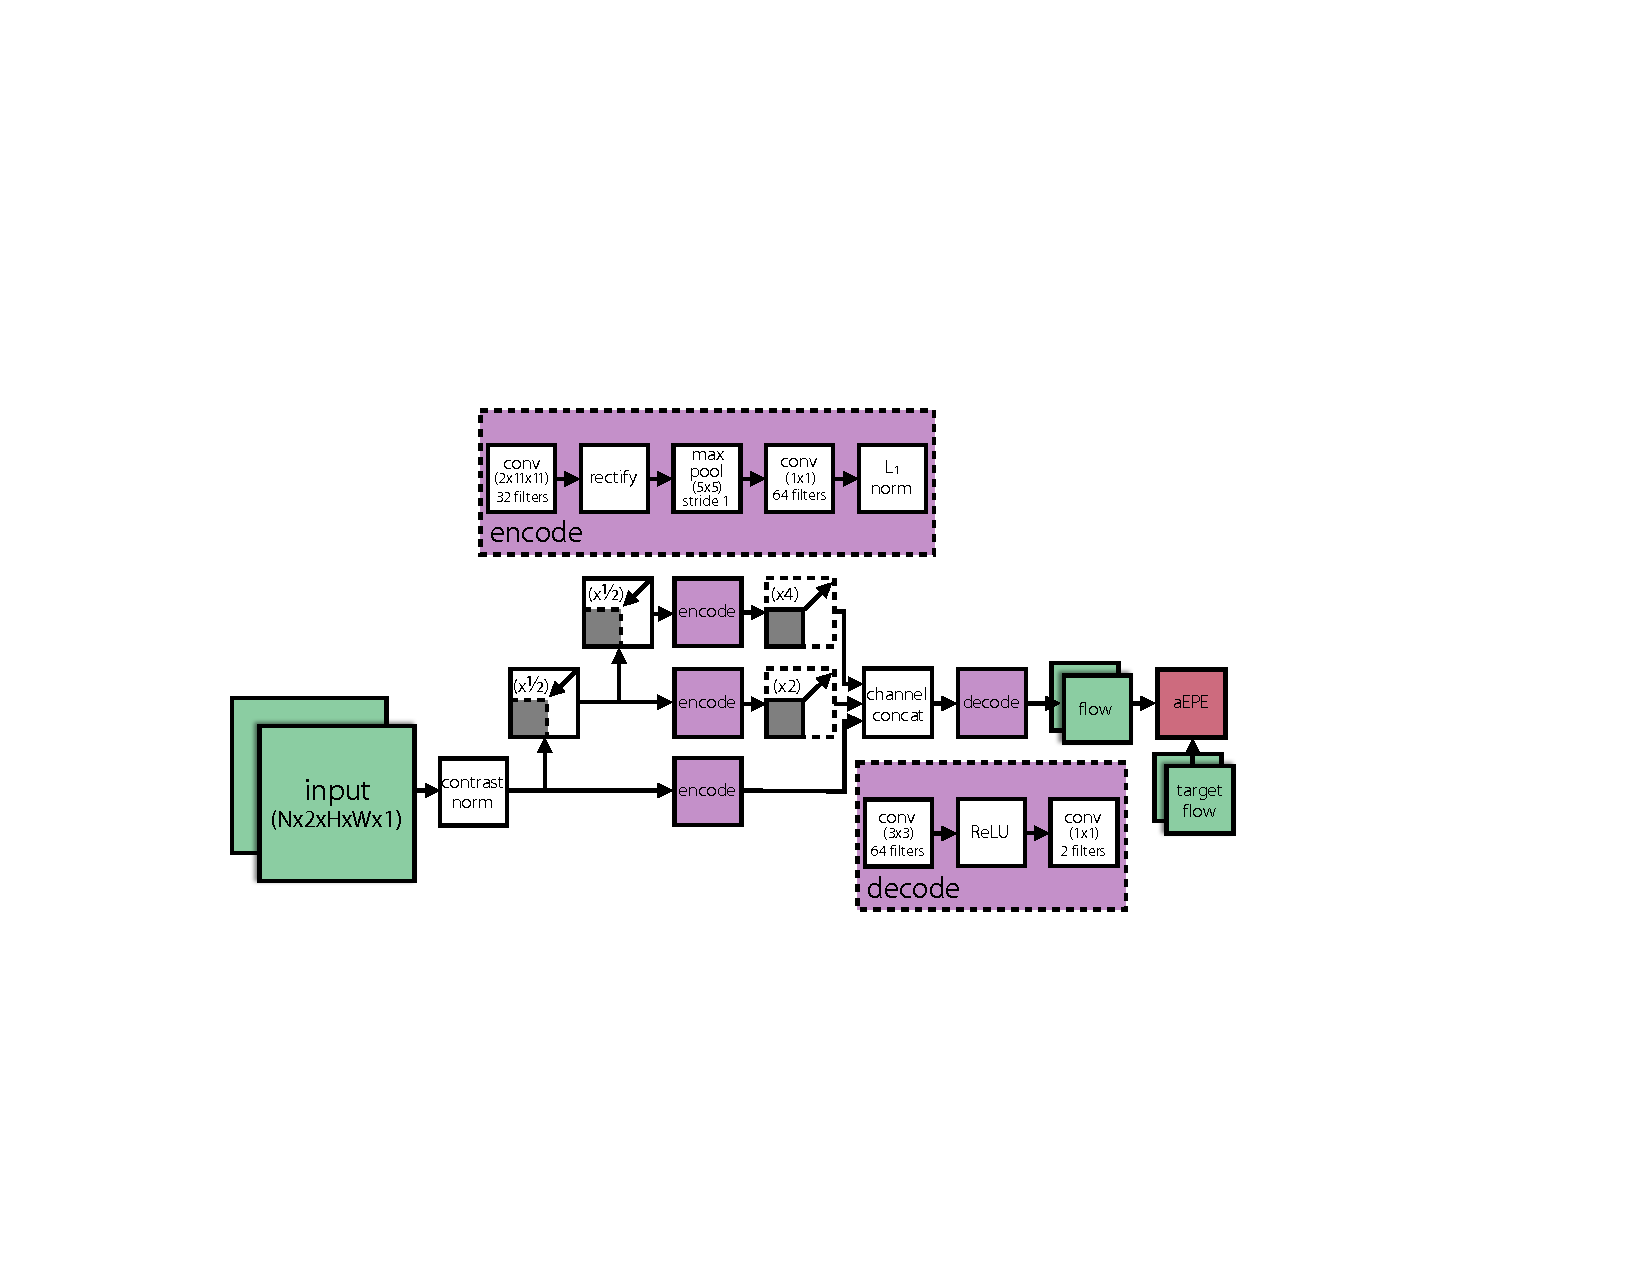
\epsfig{file=MSOEnet.pdf, width = \textwidth}
\end{center}
\vspace{-0.45cm}
\caption[Dynamics stream ConvNet.]{Dynamics stream ConvNet. The ConvNet is based on a
spacetime-oriented energy model
\cite{derpanis2012spacetime, simoncelli1998} and is trained
for optical flow prediction.
Three scales are shown for illustration;
in practice five scales are used.}
\label{fig:MSOE}
\end{figure}

For training, the standard average
endpoint error (aEPE) flow metric (\ie, $\text{L}_2$
norm) is used between the predicted flow and the ground truth
flow as the loss.
Since no large-scale optical flow dataset exists that captures
natural imagery with groundtruth flow, the assembly of a new dataset was necessary. Videos
from an unlabeled video dataset are fed through an existing flow
estimator to produce optical
flow groundtruth for training,
\cf \cite{tran2016}.
For the unlabeled video dataset, the UCF101
dataset for action recognition \cite{soomro2012ucf101} is used as it contains a wide variety of complex movements of natural imagery. The synthetic Flying Chairs dataset \cite{dosovitskiy2015} was also considered as it contained ground truth optical flow; however, training the dynamics stream on this dataset reduced the overall quality of synthesized dynamic textures. This can be explained by the limited motions and appearances exhibited by the rigid objects in Flying Chairs, which is undesirable for estimating motion of dynamic textures.
For producing the optical flow groundtruth, the EpicFlow \cite{revaud2015epicflow} model is used for 
its state-of-the-art performance (at the time of experimentation) on optical flow \edit{prediction}{estimation}.

The distribution of movement directions in UCF101 is biased to left-to-right and right-to-left motions, which is undesirable as dynamic textures are not necessarily restricted to certain directions of motion. To combat this dataset bias, geometric data augmentations similar to those used by FlowNet \cite{dosovitskiy2015} are used to equalize the distribution of movement directions in the generated dataset. Additionally, photometric data augmentations similar to those used by FlowNet \cite{dosovitskiy2015} are used here as well. These augmentations include an image rotation with a rotation amount uniformly sampled from the range $[-180 \degree , 180 \degree]$; left-right and up-down flipping with a $50\%$ chance; additive gaussian noise with a sigma uniformly sampled from the range $[0, 0.04*255]$; gamma correction with a gamma value uniformly sampled from the range $[0.7, 1.5]$; additive brightness change with the additive value normally sampled from the distribution $\mathcal{N}(\mu = 0, \sigma = 0.2*255)$; and a multiplicative brightness change with the multiplicative value uniformly sampled from the range $[0.2, 1.4]$. Each of these augmentations are done in random order.
The aEPE loss is optimized using Adam \cite{kingma2017}.

\highlight{Optical flow is chosen as the proxy task (as opposed to dynamic texture recognition \cite{derpanis2012spacetime}) for learning the distributed representation of dynamics (\ie, the first layer filters) because of the ease of obtaining large amounts of optical flow groundtruth for training. Although optical flow is not a suitable representation of the dynamics in dynamic textures, it is sufficient enough to induce the encoding stage to learn a bank of spacetime-oriented filters as the first layer of filters.}
\highlight{Furthermore,} inspection of the learned filters in the initial layer of the encoding stage
showed evidence of spacetime-oriented filters, consistent with
the handcrafted filters used in previous work \cite{derpanis2012spacetime}. This \highlight{point} is illustrated in Fig.\ \ref{fig:filters}.

\begin{figure}
	\centering
	\begin{subfigure}[b]{0.25\textwidth}
	    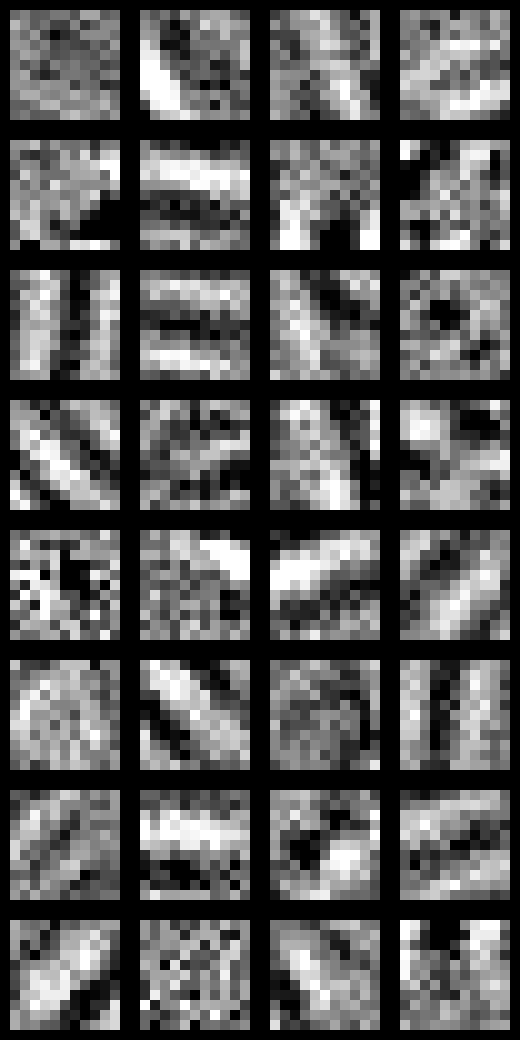
\epsfig{file=MSOEnet_filters_1.png, width = \textwidth}
		\vspace{-0.45cm}
		\caption{Frame 1}
	\end{subfigure}\hspace{5mm}%
	\begin{subfigure}[b]{0.25\textwidth}
	    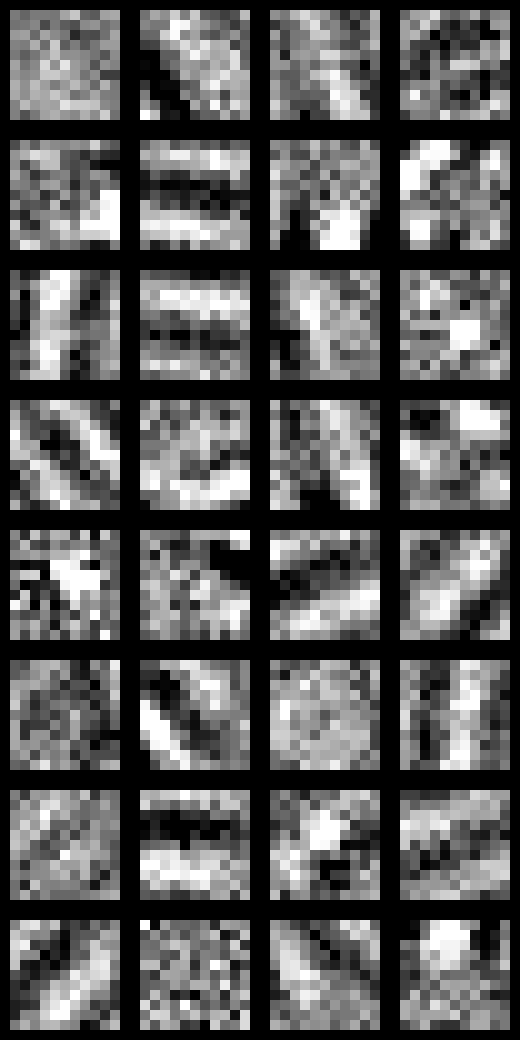
\epsfig{file=MSOEnet_filters_2.png, width = \textwidth}
		\vspace{-0.45cm}
		\caption{Frame 2}
	\end{subfigure}
	\caption[Learned spacetime-oriented filters]{32 learned spacetime-oriented filters of size $2 \times 11 \times 11$. (a) and (b) each depict a temporal slice of the learned filters, operating on the first and second frame of an input pair, respectively. Inspection of the learned filters reveals structures consistent with the handcrafted temporal derivative filters used in previous work \cite{derpanis2012spacetime} (\eg, row 4, col 1 captures up-right movement and row 8, col 1 captures down-right movement).}
	\label{fig:filters}
\end{figure}

\subsection{Target texture dynamics}

Similar to the appearance stream, filter response correlations
in a particular layer of the dynamics
stream are averaged over the number of image frame
pairs and encapsulated by a Gram matrix,
$\mathbf{G}^{l} \in \mathbb{R}^{N_l \times N_l}$,
whose entries are given by:
\begin{equation}
	G_{ij}^l = \frac{1}{(T-1) N_l M_l} \sum_{t=1}^{T-1} \sum_{k=1}^{M_l} D_{ik}^{l(t,\ t+1)} D_{jk}^{l(t,\ t+1)}\ ,	
\end{equation}
where $D_{ik}^{l(t,\ t+1)}$ denotes the activation of feature $i$ at
location $k$ in layer $l$ on the target frames $t$ and $t+1$.

\subsection{Synthesized texture dynamics}

The dynamics of the synthesized texture is represented
by a Gram matrix of filter response correlations 
computed separately for each pair of frames,
$\hat{\mathbf{G}}^{l(t,\ t+1)} \in \mathbb{R}^{N_l \times N_l}$,
with entries:
\begin{equation}
	\hat{G}_{ij}^{l(t,\ t+1)} = \frac{1}{N_l M_l} \sum_{k=1}^{M_l} \hat{D}_{ik}^{l(t,\ t+1)} \hat{D}_{jk}^{l(t,\ t+1)}\ ,	
\end{equation}
where $\hat{D}_{ik}^{l(t,\ t+1)}$ denotes the activation of feature $i$ at
location $k$ in layer $l$ on the synthesized frames $t$ and $t+1$.

\subsection{Dynamics loss}

The dynamics loss, $\mathcal{L}_\text{dynamics}$, is defined as
the average of the mean squared error between the Gram matrices
of the input texture
and those of the generated texture:
\begin{equation}
   \mathcal{L}_\text{dynamics} = \frac{1}{L_\text{dyn} (T_\text{out}-1)}\sum_{t=1}^{T_\text{out}-1} \sum_{l}  \Vert \mathbf{G}^l - \hat{\mathbf{G}}^{l(t,\ t+1)}\Vert^2_F\ , \label{eq:dynloss}
\end{equation}
where $L_\text{dyn}$ is the number of ConvNet layers being used
in the dynamics stream to compute Gram matrices.

The Gram matrix is computed on the output of the concatenation layer,
where the multiscale distributed representation of orientations is
stored. While it is tempting to use the predicted optical flow output from the
network's decoder stage, this generally yields poor results as shown in the evaluation.
Due to the complex, temporal variation present in dynamic
textures, they contain a variety of local spacetime
orientations rather than a single dominant orientation.
As a result, the flow estimates will tend to be an average of the
underlying  orientation measurements and consequently not
descriptive. A comparison between the texture synthesis results using the concatenation layer and the predicted flow output is provided in Chapter \ref{chap:evaluation}.

\section{Dynamic texture synthesis}\label{sec:texgen}
The overall dynamic texture loss consists of the combination of the appearance loss, Eq.\ (\ref{eq:apploss}),
and the dynamics loss, Eq.\ (\ref{eq:dynloss}):
\begin{equation}
   \mathcal{L}_\text{dynamic texture} = \alpha\mathcal{L}_\text{appearance} + \beta \mathcal{L}_\text{dynamics}\ , \label{eq:dyntexloss}
\end{equation}
where $\alpha$ and $\beta$ are the weighting factors for the
appearance and dynamics content, respectively. \highlight{They are set to $1\mathrm{e}{9}$ and $1\mathrm{e}{15}$, respectively.}
Dynamic textures are implicitly defined as the (local) minima 
of this loss.
Textures are generated by optimizing Eq.\ 
(\ref{eq:dyntexloss}) with respect to the synthesized spacetime volume,
\ie, the pixels of the video.
Variations in the resulting texture are found by initializing the
optimization process using IID Gaussian noise.
Consistent with previous work \cite{gatys2015}, L-BFGS \cite{liu1989} is used for optimization. Dynamic texture synthesis results are provided in Chapter \ref{chap:evaluation}.

\subsection{Incremental texture synthesis}\label{sec:incremental_synthesis}

Naive application of the outlined approach will consume
increasing amounts of memory (in this case, GPU memory) used by the ConvNet as the temporal extent (\ie, number of frames) of the 
dynamic texture grows; this \highlight{fact} makes it impractical to process and generate longer sequences.
Instead, long sequences can be incrementally generated by
separating the sequence into subsequences and optimizing them 
sequentially. Fig.\ \ref{fig:incremental_synthesis}
shows a visualization of the incremental texture synthesis process.

This \highlight{process} is realized by initializing the first frame of a subsequence as the last 
frame from the previous subsequence and keeping it fixed throughout
the optimization.
The remaining frames of the subsequence are initialized randomly and
optimized as above.
This \highlight{approach} ensures temporal consistency across synthesized subsequences
and can be viewed as a form of coordinate descent for the full
sequence objective. \highlight{Specifically, each subsequence can be viewed as a coordinate/direction of the full sequence objective that is to be minimized over, while keeping the other coordinates (\ie, other subsequences) fixed.} This \highlight{approach} can also be viewed as a form of non-linear autoregression where the output variable (in this case, the current subsequence) non-linearly depends on its previous values (previously synthesized subsequence) and a stochastic term (randomly initialized frames of the current subsequence).
The flexibility of this framework allows other texture generation
problems to be handled simply by altering the 
initialization of frames and controlling which
frames or frame regions are updated.

\begin{figure}[t]
	\centering
    
\epsfig{file=incremental_synthesis.pdf, width = 0.9\textwidth}
	\caption[Incremental texture synthesis.]{Incremental texture synthesis.
	Long sequences can be incrementally generated by
separating the sequence into subsequences and optimizing them 
sequentially. The last frame (red) of a previously synthesized subsequence
(left) is used to initialize the first frame of the next subsequence (middle)
and is kept fixed throughout optimization. The remaining frames of the 
subsequence (green) are initialized randomly and optimized as per usual.
Finally, the two subsequences are combined to produce a longer
sequence (right).}
	\label{fig:incremental_synthesis}
\end{figure}



\subsection{Temporally-endless texture synthesis}\label{sec:temporally_endless_synthesis}

An interesting extension that was explored were dynamic textures where there is no discernible temporal seam between the last and first frames. Played as a loop, these textures appear to be temporally endless. This is trivially achieved by adding an additional term to the dynamics loss (Eq.\ \ref{eq:dynloss}) that ties the last frame to the first:
\begin{equation}
	\mathcal{L}_\text{dynamics} = \frac{1}{L_\text{dyn} T_\text{out}}\left(\sum_{t=1}^{T_\text{out}-1} \sum_{l}  \Vert \mathbf{G}^l - \hat{\mathbf{G}}^{l(t,\ t+1)}\Vert^2_F + \sum_{l}  \Vert \mathbf{G}^l - \hat{\mathbf{G}}^{l(T_\text{out},\ 1)}\Vert^2_F\right).
\end{equation}

\subsection{Dynamics style transfer}

The underlying assumption of the proposed model is that the appearance
and dynamics of dynamic textures can be factorized.
As such, it should allow for the transfer of the dynamics of
one texture onto the appearance of another.
This \highlight{operation} has been explored previously for image style transfer
\cite{champandard2016,gatys2017} with static imagery.
\edit{This}{The operation} is accomplished with the proposed model by performing the same 
optimization as described in Sec.\ \ref{sec:texgen}, but with the target Gram matrices for 
appearance and dynamics computed from two different textures, respectively.

\section{Summary}

This chapter presented the technical approach of the proposed ConvNet for dynamic texture synthesis, including its various extensions. The ConvNet implemented a factored approach in separately modelling the appearance (\ie, spatial content) and dynamics information (\ie, temporal variation) of an input dynamic texture. It consisted of two main components: an appearance stream and a dynamics stream. Each stream consisted of a ConvNet whose activation correlations (\ie, Gram matrices) were used to characterize the dynamic texture. The appearance stream was an adaptation of the static texture model introduced by Gatys \etal \cite{gatys2015}. Here it was utilized by applying it independently to each frame of the dynamic texture, arriving at a purely appearance-wise description of it.

Parallel to the appearance stream is the dynamics stream, which was designed for purely capturing texture dynamics while forgoing appearance. Dynamic textures exhibit complex temporal variations that can not be adequately modelled by optical flow alone. Thus, a novel ConvNet was proposed, taking inspiration from spacetime-oriented energy models \cite{derpanis2012spacetime,simoncelli1998} that can characterize temporal imagery beyond the capabilities of optical flow. Namely, the Marginalized Spatiotemporal Oriented Energies (MSOE) model introduced by Derpanis and Wildes \cite{derpanis2012spacetime} was adapted to a ConvNet, which was trained through the proxy task of predicting optical flow.

Dynamic textures were synthesized by optimizing each stream's objective with respect to the synthesized texture. Both streams followed the objective of minimizing the distances between activation correlations of the synthesized dynamic texture and target dynamic texture.

Finally, this chapter presented three extensions to the proposed model: incremental texture synthesis, temporally-endless texture synthesis, and dynamics style transfer. Incremental texture synthesis provided a solution to memory-constraints brought upon by the synthesis of long dynamic textures by introducing an incremental synthesis process over subsequences of the entire dynamic texture. Temporally-endless texture synthesis included an additional constraint on the dynamics objective that tied the last and first frame of the synthesized dynamic texture, producing dynamic textures that appeared to be endlessly looping. Dynamics style transfer took advantage of the two-stream factorization of appearance and dynamics to synthesize dynamic textures that combine the texture appearance from one target with the dynamics from another.